%----------------------------------------------------------------------------------------
%	Literature research
%----------------------------------------------------------------------------------------
\chapter{Literature research} % Main chapter title
\label{Chapter2} % For referencing the chapter elsewhere, use \ref{Chapter2}

This chapter covers the in-depth research conducted on up-grade martial arts and examines the suitability of off-the-shelf software solutions for customer relationship management for the business.

%----------------------------------------------------------------------------------------
%	1. Company research
%----------------------------------------------------------------------------------------

\section{Company research}
Building a bespoke system requires tailoring to the business and its operations. Therefore, information gathering was essential to ensure the new software fits within their ecosystem. 

\subsection{Meetings}

Research began through an initial meeting with the business owners. In this session, we discussed their problem and potential solutions. The final solution was to develop a single system accessible from any location that unifies the data storage and searching of business-critical data.


\begin{table}[ht!]
    \renewcommand{\arraystretch}{1.5}
    \label{fig:meetingtable}
    \caption{Problems the business faces and the proposed solutions}
    \centerline{
        \begin{NiceTabular}{ m{4.5cm} m{3.6cm} m{4.5cm}  }
            \hline
            \textbf{Problem} & \textbf{Domain} & \textbf{Solution}\\
            \hline \hline
            Fragmented system & Operational & Condense all processes into a single system \\
            \hline
            Slow member signup & Functional & Create digital signup \\
            \hline
            Inconsistent input & Data & Standardised input display and method \\
            \hline
            Slow member search & Health and Safety & Create easy lookup through table \\
            \hline
            Statistics takes too long to calculate & Business & Have stats calculated on-the-fly clearly visible \\
            \hline
            No method of cross-referencing member attendance with payments & Financial & Use a token system which are valid for single use across a time range \\
            \hline
           \end{NiceTabular}
    }
\end{table}


\subsection{User stories}
In subsequent discovery sessions, requirements, user stories and wireframes were created to consolidate the system's operations and boundaries, preventing feature creep.

\begin{table}[ht!]
    \renewcommand{\arraystretch}{1.2}
    \label{fig:userstories}
    \caption{User stories}
    \centerline{
        \begin{NiceTabular}{ m{3.3cm} m{4.6cm} m{5cm}  }
            \hline
            \textbf{Action} & \textbf{Process} & \textbf{Result}\\
            \hline \hline
            Login & Validate and verify details & Provide or deny access to the system \\
            \hline
            View members & Go to members page & Table showing all members. Click reveals all detials \\
            \hline
            Add members & Go to members page, fill in form, submit & New member shows in table \\
            \hline
            Edit members & Go to members page, click member to edit, update and submit & Member details update in table \\
            \hline
            View Lessons & Go to lessons page & Table showing all lessons. Click reveals all detials \\
            \hline
            Add Lessons & Go to lessons page, fill in form, submit & New lesson shows in table \\
            \hline
            Edit Lessons & Go to lessons page, click member to edit, update and submit & Lesson details update in table \\
            \hline
            View Attendance & Go to attendance page, select lessons & Table showing all attendances for selected lesson \\
            \hline
            Add Attendance Free & Go to attendance page, select lesson, select member, click add & Attendance added \\
            \hline
            Add Attendance Pay Now & Go to attendance page, select lesson, select member, click add & Payment prompted, pay now selected \\
            \hline
            Add Attendance Pay Later & Go to attendance page, select lesson, select member, click add & Payment promoted, pay later selected \\
            \hline
            View bulk purchase & Go to purchase page & Table showing all prices for lessons \\
            \hline
            Add bulk purchases & Go to purchase page, select member, select purchase plan & confirm payment, log transaction \\
            \hline
            View Payments & Go to payments page & Table showing all payments for all lessons \\
            \hline
            View statistics & Go to dashboard page & All statistics viewable in single page \\
            \hline
           \end{NiceTabular}
    }
\end{table}


\subsection{Document acquisition}
Document acquisition was also a crucial part of the research. Publicly available resources were collected alongside internal material. Documents included price lists (Appendix \ref{AppendixC:PriceList}), member signup form (Appendix \ref{AppendixC:SignupForm}) and attendance spreadsheets (Appendix \ref{AppendixC:AttendanceSpreadsheet}). The personally identifiable information was redacted, so only the structures remained.

Copyrighted content, such as logos and colour schemes from their website, would heavily influence the design. Consequently, written permission was requested from all business owners and was confirmed at the beginning of development (Figure~\ref{fig:consent}).

\begin{figure}[ht!]
    \centerline{\fbox{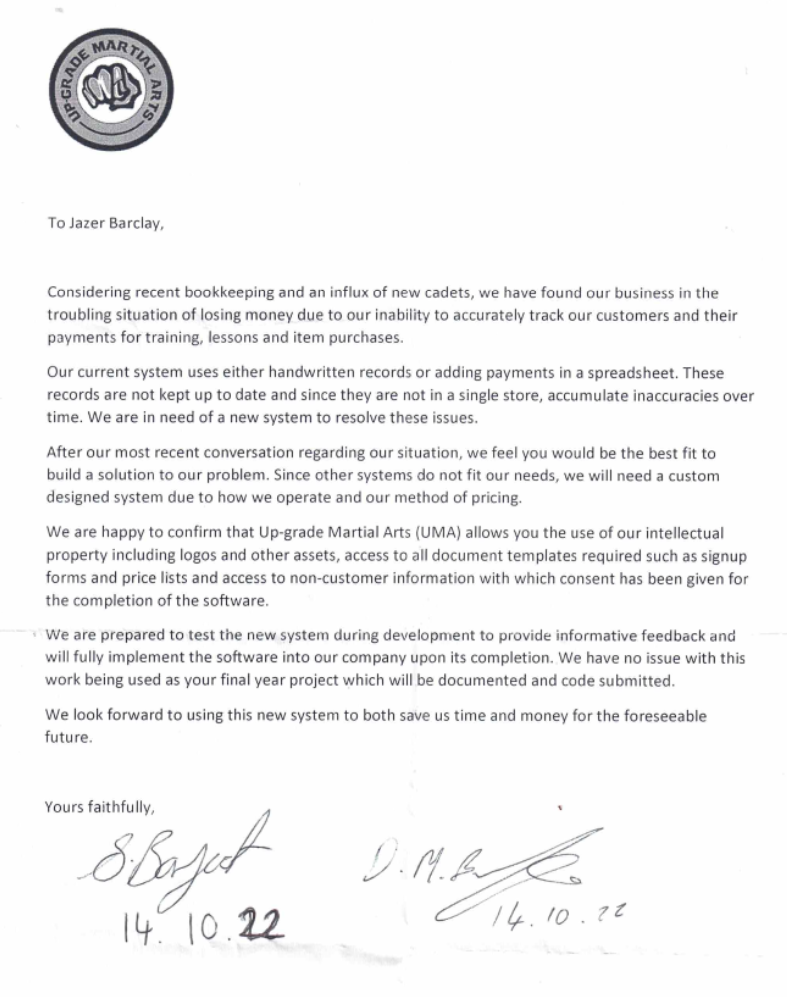
\includegraphics[width=.75\linewidth]{consent.png}}}
    \caption{Consent to create the application and use business copyrighted assets during development}
    \label{fig:consent}
\end{figure}


\subsection{Results of research}
The in-depth research into the business reveals a system that started small with new elements and features added without considering expansion over time. The fragmented nature creates friction between the end user and the data.

%----------------------------------------------------------------------------------------
%	2. Competitor analysis
%----------------------------------------------------------------------------------------

\section{Competitor analysis}
Off-the-shelf customer relationship management software exists for general-purpose use. These are designed for small to medium-sized businesses with a more generic approach to business operations.

The leading software in the space are InvoiceNinja \parencite{noauthor_invoice_nodate} and HubSpot \parencite{noauthor_hubspot_2022}. Both boast being free with premium pricing plans for access to more advanced and comprehensive tools, many of which the business requires.

UMA has tested many CRM and Point-of-Sale (PoS) systems in the past; however, due to their complex pricing and lesson structure, many fall short of their extensive requirements or require two separate systems to operate.

Attempts to use this software have resulted in even greater confusion, and business data has become fragmented across all systems.

A more critical study compared and contrasted the leading software currently on the market to further the research into existing software found in Table~\ref{fig:soft-comp}.

\begin{table}[ht!]
    \caption{Off-the-shelf software comparison based on features}
    \renewcommand{\arraystretch}{2}
    \centerline{
        \begin{NiceTabular}{ m{2.2cm} m{4cm} m{4cm} m{2cm}  }
            \hline
            \textbf{Feature} & \textbf{HubSpot} & \textbf{Invoice Ninja} & \textbf{Best Fit}\\
            \hline \hline
            Customer input & Complex to setup however supports the required field very well & Easy to input however limited on fields available & Both\\
            \hline
            Customer search & Advanced search tools available but requires setup & Simple search based on fixed fileds & HubSpot\\
            \hline
            Purchase tracking & Setup is required but does a good job & Very good providing useful tools and analytics & Invoice Ninja\\
            \hline
            Service tracking & Services need configuration which is not as straight forward & Services are treated like good making input and tracking easy & Invoice Ninja\\
            \hline
            Multi-lesson purchasing & Was unable to configure this within the system & Does not support functionality to configure this & Neither\\
            \hline
            Data insights & Good analytical data but, again, requires custom configuration & Since the structure of the system is quite fixed, very good analytics on the structures it provides & Both \\
            \hline
           \end{NiceTabular}
    }
    \label{fig:soft-comp}
\end{table}

InvoiceNinja focuses more on customer data storage and pricing, whereas HubSpot is designed for customer interaction through marketing and sales.

\begin{figure}[ht!]
    \centerline{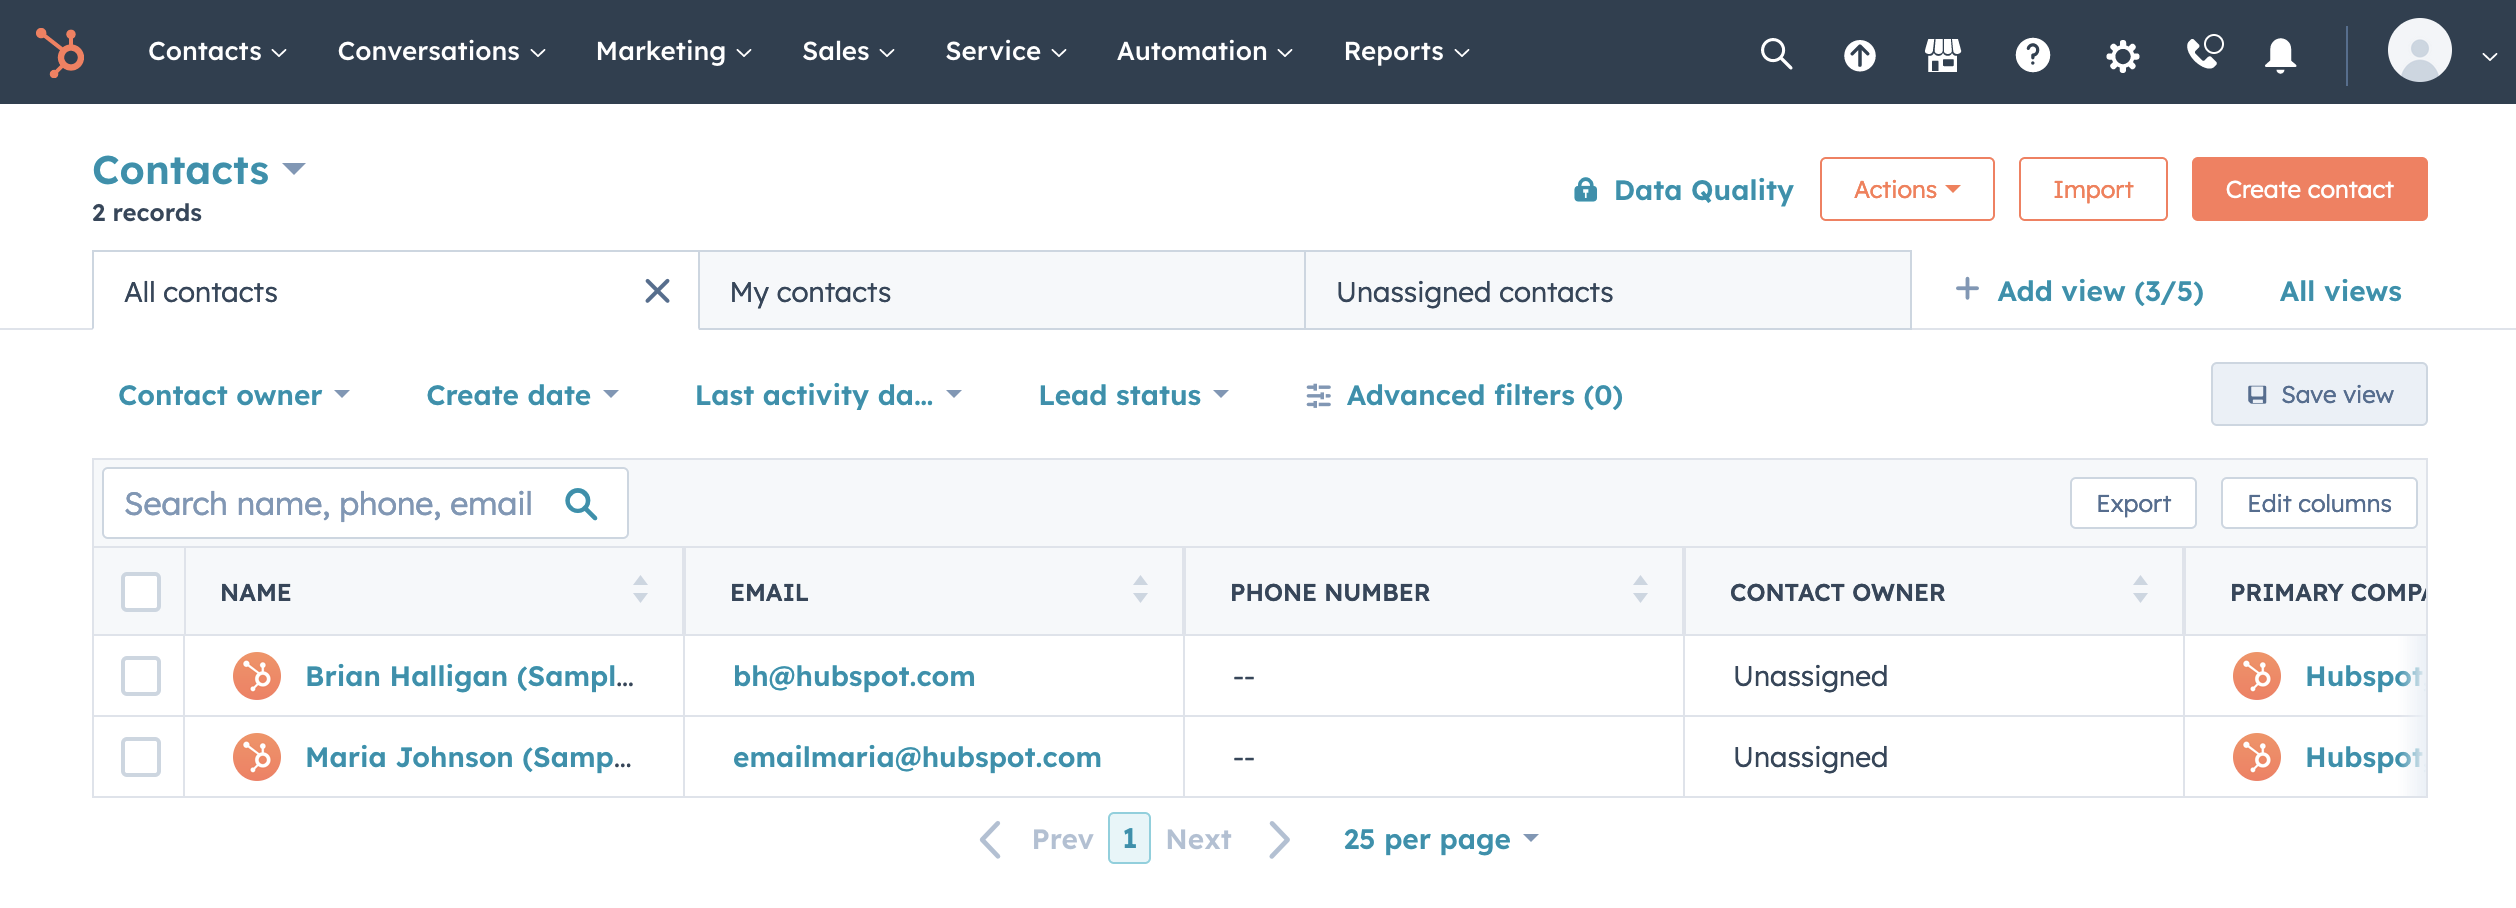
\includegraphics[width=\linewidth]{hubspot.png}}
    \caption{HubSpot customer management panel}
    \label{fig:hubspot}
\end{figure}

They both support handling customer data and tracking purchases. However, HubSpot better visualises this data by providing a more customisable, modular dashboard. On the other hand, Invoice Ninja allows for easier data entry and lookup through their simple interface.

\begin{figure}[ht!]
    \centerline{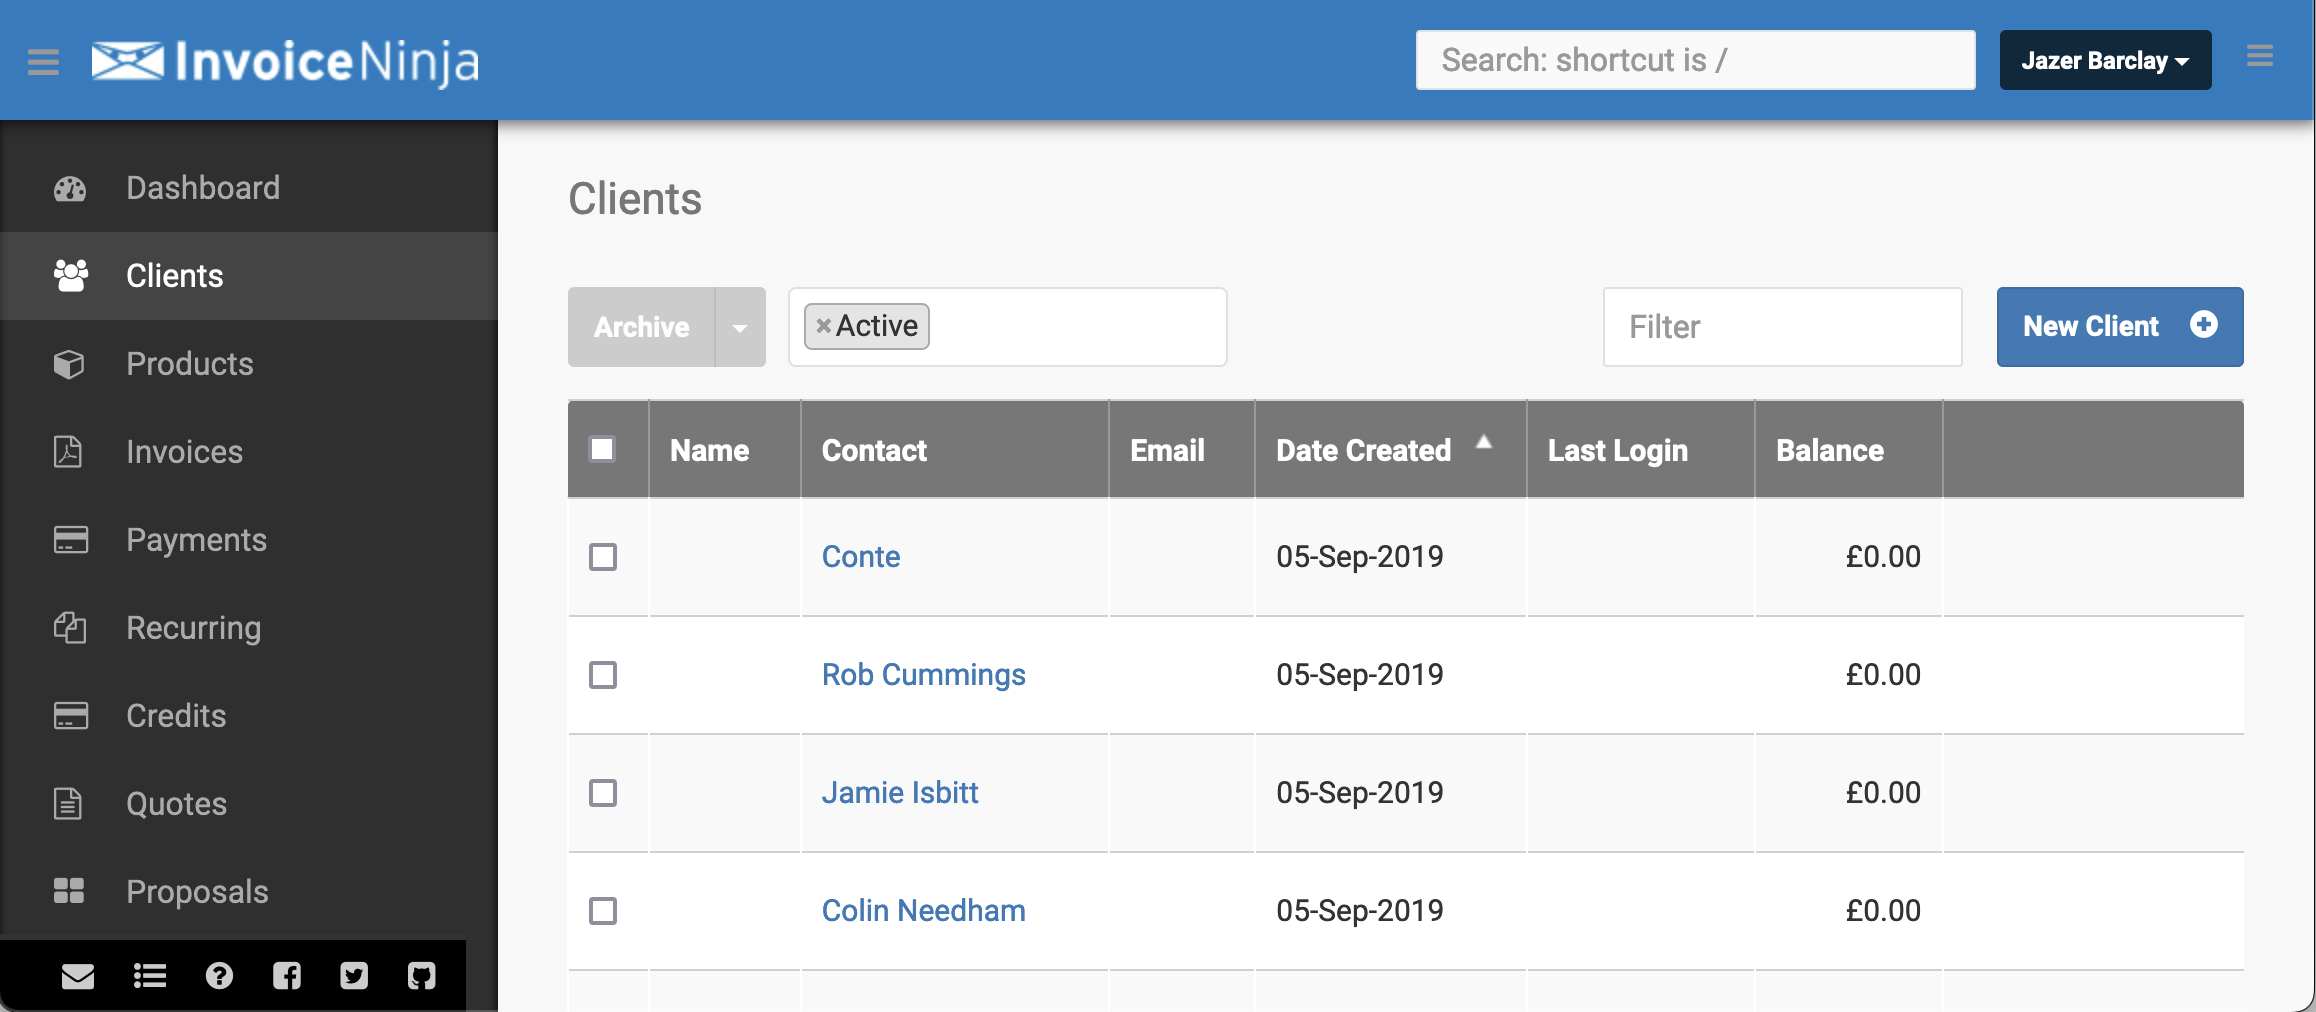
\includegraphics[width=\linewidth]{invoiceninja-customers.png}}
    \caption{Invoice Ninja customer management panel}
    \label{fig:invoiceninja}
\end{figure}

Invoice Ninja meets many more requirements than HubSpot, especially those the business requires, such as efficiently handling customer data entry and lookup. It also supports various products and services, which can be billed as an invoice or purchase.

Where both of these disappoint are in the pricing and lesson purchase models. Neither supports more complex purchase tracking or pricing, which the business needs to prevent further financial losses.

In summary, both software systems provide only some of the system requirements. Nonetheless, no single software covers them all, and neither solves the core issue that the business faces, which involves attendance and payment tracking. Since the primary off-the-shelf software cannot satisfy the requirements, the solution to their problems is within a custom and bespoke system.